% !TeX program = pdflatex
\documentclass[tikz,border=8pt]{standalone}
\usepackage{tikz}
\definecolor{FigureBlue}{HTML}{2563EB}\definecolor{FigureOrange}{HTML}{EA580C}
\begin{document}
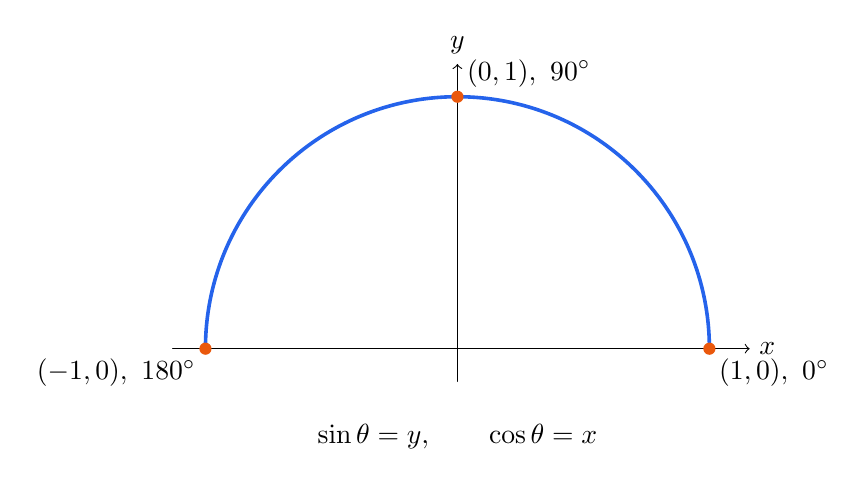
\begin{tikzpicture}[x=3.2cm,y=3.2cm,line cap=round]
  \draw[->] (-1.13,0)--(1.16,0) node[right] {$x$}; \draw[->] (0,-.13)--(0,1.13) node[above] {$y$};
  \draw[FigureBlue,line width=1.3pt] (1,0) arc[start angle=0,end angle=180,radius=1];
  \fill[FigureOrange] (1,0) circle (2.2pt); \node[below right] at (1,0) {$(1,0),\ 0^\circ$};
  \fill[FigureOrange] (0,1) circle (2.2pt); \node[above right] at (0,1) {$(0,1),\ 90^\circ$};
  \fill[FigureOrange] (-1,0) circle (2.2pt); \node[below left] at (-1,0) {$(-1,0),\ 180^\circ$};
  \node at (0,-.35) {$\sin\theta=y,\qquad \cos\theta=x$};
\end{tikzpicture}
\end{document}
